\chapter{定量分析的数理基础}

\section{数学}
定量研究对于不少文科专业的同学来说最关键的一个门槛便是理解数学公式,好在笔者本人也是文科专业出身,写这一部分足够契合(水平也菜)。

本文介绍了因果推断中常用的数学基础,包括微积分、线性代数、概率与分布、以及统计推断等内容。这些基础知识为理解和应用因果推断方法提供了必要的数学工具。

\subsection{微积分}

\paragraph*{函数}
在数学中,函数是一种特殊的关系,它将一个集合中的每个元素(\textbf{自变量})映射到另一个集合中的唯一元素(\textbf{因变量})。函数可以用多种方式表示,包括解析式、图像、表格和算法等。函数的概念在微积分中至关重要,因为微积分的主要研究对象就是函数的变化率和累积量。

\paragraph*{导数}
一元函数 $ y = f(x) $ 的一阶导数定义为:
\begin{equation}
\frac{\mathrm{d}y}{\mathrm{d}x} \equiv f'(x) \equiv \lim_{\Delta x \to 0} \frac{\Delta y}{\Delta x} \equiv \lim_{\Delta x \to 0} \frac{f(x + \Delta x) - f(x)}{\Delta x}
\end{equation}

\noindent 其几何意义是函数在某点的切线斜率。二阶导数定义为:
\begin{equation}
\frac{\mathrm{d}^2y}{\mathrm{d}x^2} \equiv f''(x) \equiv [f'(x)]'\equiv \frac{\mathrm{d}\left(\frac{\mathrm{d}y}{\mathrm{d}x}\right)}{\mathrm{d}x}
\end{equation}
\noindent 二阶导数反映了函数图像切线斜率的变化率,描述了曲线的弯曲程度,这一性质在数学中被称为\textbf{曲率(curvature)}。在经济学中,我们一般默认二阶导数恒为正或负值。

\begin{figure}[ht]
	\centering
	\fbox{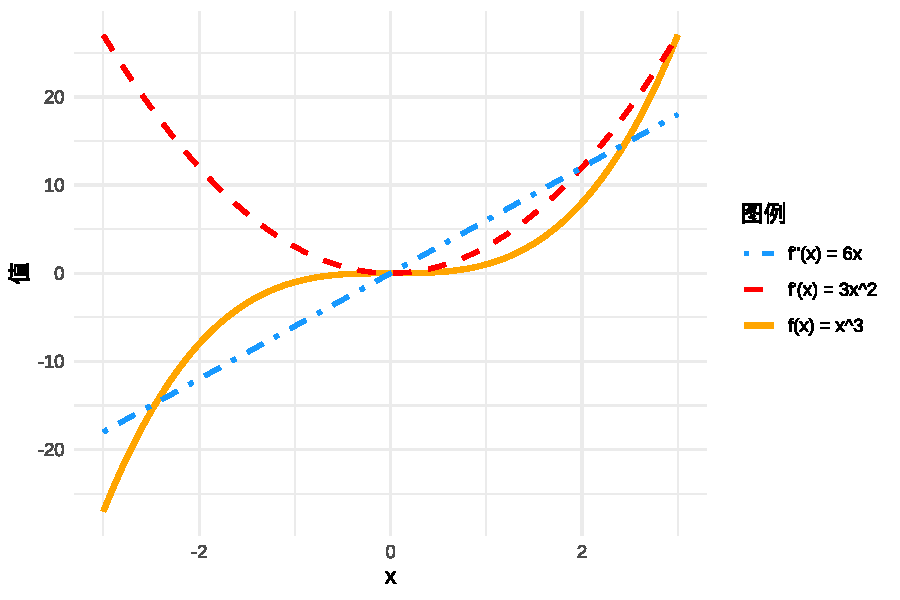
\includegraphics[width=0.5\textwidth]{image/f2.pdf}}
	\caption{函数 $f(x) = x^3$ 与其一阶、二阶导数}
\end{figure}

\paragraph*{偏导数}
偏导数是多元函数对其中一个变量的导数,而将其他变量视为常数。例如,对于二元函数 \( y = f(x, z) \),其对 \( x \) 的偏导数定义为:
\begin{equation}
	\frac{\partial y}{\partial x} \equiv \lim_{\Delta x \to 0} \frac{f(x + \Delta x, z) - f(x, z)}{\Delta x}
\end{equation}
\noindent 类似地,对 \( z \) 的偏导数为:
\begin{equation}
	\frac{\partial y}{\partial z} \equiv \lim_{\Delta z \to 0} \frac{f(x, z + \Delta z) - f(x, z)}{\Delta z}
\end{equation}
\noindent 偏导数在经济学中有着广泛的应用,例如在效用函数和生产函数中,偏导数分别表示商品和生产要素的边际效应。

\paragraph*{基本求导规则}

\begin{itemize}
	\item 线性法则:$(cf)' = c f'$, 其中$c$为常数;
	\item 乘法法则:$(fg)' = f'g + fg'$;
	\item 除法法则:$\left(\dfrac{f}{g}\right)' = \dfrac{f'g - fg'}{g^2}$;
	\item 链式法则:$(f(g(x)))' = f'(g(x)) \cdot g'(x)$。
\end{itemize}

\begin{table}[h]
	\centering
	\caption{常见函数的导数公式}
	\renewcommand{\arraystretch}{2}
	\begin{tabularx}{\linewidth}{>{\centering\arraybackslash}X >{\centering\arraybackslash}X}
		\toprule
		函数 & 导数 \\
		\midrule
		常数 $c$         & $0$ \\
		$x^n$            & $n x^{n-1}$ \\
		$\sin x$         & $\cos x$ \\
		$\cos x$         & $-\sin x$ \\
		$e^x$            & $e^x$ \\
		$a^x$            & $a^x \ln a$ \\
		$\ln x$          & $\dfrac{1}{x}$ \\
		$\log_a x$       & $\dfrac{1}{x \ln a}$ \\
		$\tan x$         & $\sec^2 x$ \\
		\bottomrule
	\end{tabularx}
\end{table}

\paragraph*{洛必达法则}
洛必达法则的核心思想是通过分子分母分别求导,解决$\frac{0}{0}$或$\frac{\infty}{\infty}$型不定式极限问题:
\begin{equation}
	\lim_{x \to c} \frac{f(x)}{g(x)} = \lim_{x \to c} \frac{f'(x)}{g'(x)} \quad \text{(若满足条件)}
\end{equation}
适用条件包括:极限形式为$\frac{0}{0}$或$\frac{\infty}{\infty}$,$f(x), g(x)$在$c$的去心邻域内可导且$g'(x) \neq 0$,求导后极限存在或为无穷。

\vspace{0.8em} % 手动调整间距

\begin{example}
\noindent 证明 $\lim\limits_{x\to+\infty}\left(1+\frac{1}{x}\right)^{x}=e$
	\begin{flushleft}
		\textbf{证明思路}:通过取对数转换,构造$\frac{0}{0}$型极限,应用洛必达法则求解。
	\end{flushleft}
	\begin{flushleft}	
		\textbf{证明步骤:}
	\end{flushleft}
	\begin{enumerate}
		\item 设 $y = \left(1+\frac{1}{x}\right)^x$,取对数得 $\ln y = x\ln\left(1+\frac{1}{x}\right)$
		\item 令 $t=\frac{1}{x}$,转化为 $\lim\limits_{t\to 0^+}\frac{\ln(1+t)}{t}\ \left(\frac{0}{0}\text{型}\right)$
		\item 应用洛必达法则:
		$$
		\lim_{t\to 0^+}\frac{\ln(1+t)}{t} \overset{\text{L'H}}{=} \lim_{t\to 0^+}\frac{1/(1+t)}{1} = 1
		$$
		\item 还原得 $\lim\limits_{x\to+\infty}\ln y =1 \ \Rightarrow\ \lim\limits_{x\to+\infty} y = e^1 = e$
	\end{enumerate}
\end{example}

\paragraph*{一元最优化}
最小二乘法(OLS)和最大似然估计(MLE)都是最优化问题。无约束的一元最优化问题中,最大化问题的一阶条件为$f'(x^*) = 0$,二阶条件为$f''(x^*) \leq 0$;最小化问题的一阶条件同样为$f'(x^*) = 0$,二阶条件为$f''(x^*) \geq 0$。

\paragraph*{多元最优化}

考虑无约束的多元最大化问题:
\begin{equation}
	\max_x f(x) = f(x_1, x_2, \ldots, x_n)
\end{equation}

\noindent 其一阶条件要求在最优值 $x^*$ 处,所有偏导数均为0:

\begin{equation}
	\frac{\partial f}{\partial x_i}(x^*) = 0 \quad \text{for all } i = 1, 2, \ldots, n
\end{equation}

\noindent 该条件称为\textbf{一阶必要条件},在满足一阶条件的基础上,其充分条件为:

\paragraph*{Hessian条件}

记函数的Hessian矩阵为:
\begin{equation}
	\mathbf{H(x)} = \begin{bmatrix}
		\frac{\partial^2 f}{\partial x_1^2} & \frac{\partial^2 f}{\partial x_1 \partial x_2} & \cdots & \frac{\partial^2 f}{\partial x_1 \partial x_n} \\
		\frac{\partial^2 f}{\partial x_2 \partial x_1} & \frac{\partial^2 f}{\partial x_2^2} & \cdots & \frac{\partial^2 f}{\partial x_2 \partial x_n} \\
		\vdots & \vdots & \ddots & \vdots \\
		\frac{\partial^2 f}{\partial x_n \partial x_1} & \frac{\partial^2 f}{\partial x_n \partial x_2} & \cdots & \frac{\partial^2 f}{\partial x_n^2}
	\end{bmatrix}
\end{equation}

\begin{itemize}
	\item 若 $\mathbf{H(x^*)}$ 是\textbf{负定矩阵},则 $x^*$ 是局部极大值点。
	\item 若 $\mathbf{H(x^*)}$ 是\textbf{正定矩阵},则 $x^*$ 是局部极小值点。
	\item 若 $\mathbf{H(x^*)}$ \textbf{半正定或半负定},则可能为鞍点或边界情况。
\end{itemize}
\vspace{0.8em} % 手动调整间距

\noindent 其中,负定和正定矩阵的判定方法可通过特征值符号判断。

\begin{figure}[ht]
	\centering
	\fbox{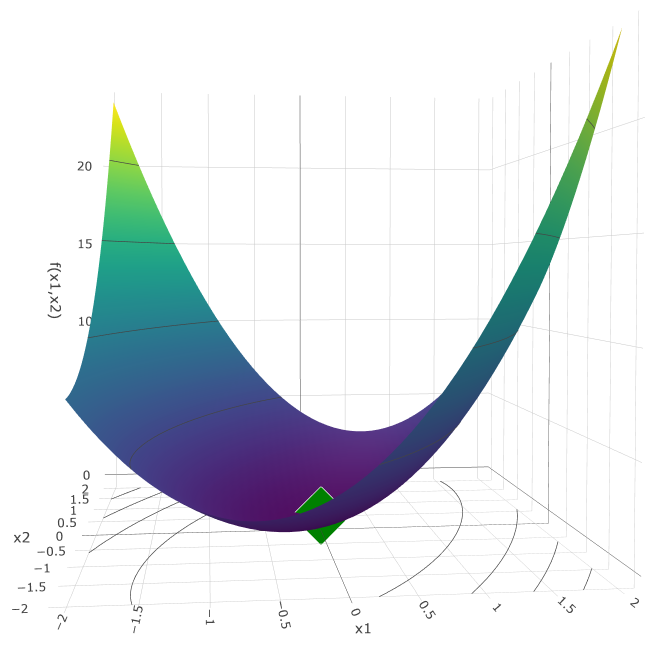
\includegraphics[width=0.5\textwidth]{image/divers.png}}
	\caption{一个抽象的多元最优化示意图}
\end{figure}

\subsection{线性代数}

\paragraph*{矩阵}
将 \( m \times n \) 个实数排列成如下矩形阵列:
\begin{equation}
\mathbf{A} = 
\begin{bmatrix}
	a_{11} & \cdots & a_{1n} \\
	\vdots & \ddots & \vdots \\
	a_{m1} & \cdots & a_{mn}
\end{bmatrix}
\end{equation}
称 \( \mathbf{A} \) 为 \( m \times n \) 级矩阵(matrix),其中:
\begin{itemize}
	\item \( m \):行数(row dimension)
	\item \( n \):列数(column dimension)
\end{itemize}

\noindent 元素 \( a_{ij} \) 表示第 \( i \) 行、第 \( j \) 列的元素。记法:\( \mathbf{A_{m \times n}} \) 或者 \( (a_{ij})_{m \times n} \)。若所有元素均为 0,则称为零矩阵(zero matrix),记作 \( \bm{0} \)。

\paragraph*{矩阵的转置}
将矩阵 \( \mathbf{A} = (a_{ij}) \) 的第 \( i \) 行变为第 \( i \) 列,得到其转置矩阵 \( \mathbf{A'} \),维度为 \( n \times m \):

\begin{equation}
	\mathbf{(A')_{ij}} = \mathbf{(A)_{ji}}
\end{equation}

\begin{itemize}
	\item 若 \( \mathbf{A} \) 是对称矩阵,则 \( \mathbf{A'} = \mathbf{A} \)
	\item 转置的转置还原:\( \mathbf{(A')'} = \mathbf{A} \)
\end{itemize}

\paragraph*{方阵}
当 \( m = n \) 时,矩阵 \( \mathbf{A} \) 称为 \( n \) 阶方阵:
\begin{equation}
\mathbf{A} = 
\begin{bmatrix}
	a_{11} & \cdots & a_{1n} \\
	\vdots & \ddots & \vdots \\
	a_{n1} & \cdots & a_{nn}
\end{bmatrix}
\end{equation}

\noindent 主对角线元素为\( a_{11}, a_{22}, \ldots, a_{nn} \)。
\begin{flushleft}
	常见类型有:
\end{flushleft}
\begin{itemize}
	\item 对称矩阵:\( a_{ij} = a_{ji} \)。
	\item 对角矩阵:非主对角线元素全为 0。
	\item 单位矩阵 \( \mathbf{I_n} \):主对角线为 1,其余为 0。
\end{itemize}

\noindent 上述三种类型的矩阵限制条件逐项增加,可以看到单位矩阵一定是对角矩阵和对称矩阵;单位矩阵 \( \mathbf{I_n} \) 在矩阵运算中作用类似于数字 1。

\paragraph*{行列式}
\begin{flushleft}
	\textbf{定义}:方阵的一个标量值函数
\end{flushleft}

\begin{itemize}
	\item 记法:$\det(\mathbf{A})$ 或 $|\mathbf{A}|$
	\item 对于 $n \times n$ 矩阵 $\mathbf{A} = (a_{ij})$:
	\begin{equation}
		\det(\mathbf{A}) = \sum_{\sigma \in S_n} \operatorname{sgn}(\sigma) \prod_{i=1}^n a_{i,\sigma(i)}
	\end{equation}
	\noindent 其中:
	\begin{itemize}
		\item $S_n$ 是 $\{1, \ldots, n\}$ 的所有排列集合
		\item $\operatorname{sgn}(\sigma)$ 是排列符号函数(偶排列为 $+1$,奇排列为 $-1$)
	\end{itemize}
\end{itemize}

\paragraph*{行列式的求解} 

\begin{flushleft}
	\textbf{定义:}
\end{flushleft}

\begin{itemize}
	\item 排列中``逆序对''的数量
	\item 举例:123(1<2<3,0),213(2>1<3,1),321(3>2>1,3)
\end{itemize}

\begin{flushleft}
	\textbf{三阶行列式展开:}
\end{flushleft}

\begin{equation}
\mathbf{D_3} = \sum (-1)^t a_{1p_1}a_{2p_2}a_{3p_3}
\end{equation}

\begin{itemize}
	\item $p_1p_2p_3$: $1,2,3$ 的排列
	\item $t$: 排列的逆序数
	\item 共6项(例如:排列 $213$ 对应 $-a_{12}a_{21}a_{33}$)
\end{itemize}

\paragraph*{n阶行列式}
\begin{equation}
	\mathbf{D_n} = \sum (-1)^t a_{1p_1} a_{2p_2} \cdots a_{np_n}
\end{equation}
\begin{itemize}
	\item $p_1 p_2 \cdots p_n$: $1$ 到 $n$ 的排列
	\item $t$: 排列的逆序数
	\item 总共 $n!$ 项(如:3阶有6项,4阶有24项)
\end{itemize}

\vspace{0.7em}
\begin{example}
	
	\noindent 设矩阵:
		\begin{equation}
		\mathbf{A} = \begin{bmatrix}
			1 & 2 & 3 \\
			4 & 5 & 6 \\
			7 & 8 & 9
		\end{bmatrix}
		\end{equation}
		
	\noindent 行列式展开:
		\begin{equation}
		\det(\mathbf{A}) = 
		1 \cdot 5 \cdot 9 + 2 \cdot 6 \cdot 7 + 3 \cdot 4 \cdot 8
		- 3 \cdot 5 \cdot 7 - 2 \cdot 4 \cdot 9 - 1 \cdot 6 \cdot 8
		\end{equation}
		
	\noindent 计算得:
		\begin{equation}
		\det(\mathbf{A}) = 45 + 84 + 96 - 105 - 72 - 48 = 0
		\end{equation}
		
	\noindent 所以:$\det(\mathbf{A}) = 0$
\end{example}

\paragraph*{向量}

\begin{flushleft}
	\textbf{定义}:若 \( m = 1 \),矩阵 \( \mathbf{A} \) 称为 \( n \) 维行向量(row vector);若 \( n = 1 \),则称为 \( m \) 维列向量(column vector)。向量是矩阵的特例。
\end{flushleft}


\begin{flushleft}
	设列向量:
\end{flushleft}

\begin{equation}
\mathbf{a} = \begin{bmatrix} a_1 \\ \vdots \\ a_n \end{bmatrix},\quad
\mathbf{b} = \begin{bmatrix} b_1 \\ \vdots \\ b_n \end{bmatrix}
\end{equation}

\begin{flushleft}
	它们的内积(点乘)定义为:
\end{flushleft}

\begin{equation}
	\begin{aligned}
		\mathbf{a}'\mathbf{b} &\equiv 
		\begin{pmatrix} a_1 & \cdots & a_n \end{pmatrix}
		\begin{pmatrix} b_1 \\ \vdots \\ b_n \end{pmatrix} \\
		&= a_1 b_1 + \cdots + a_n b_n = \sum_{i=1}^{n} a_i b_i
	\end{aligned}
\end{equation}

\begin{flushleft}
	\textbf{向量正交性}
\end{flushleft}


\begin{flushleft}
	\textbf{定义}:若 \( \mathbf{a}'\mathbf{b} = 0 \),称 \( \mathbf{a} \) 与 \( \mathbf{b} \) 正交,即在 \( n \) 维空间中相互垂直。任何形如 $\sum_{i=1}^{n} a_i b_i$ 的乘积求和,都可以很方便地写为向量内积 $a'b$ 的形式。特别地,平方和 $\sum_{i=1}^{n} a_i^2$ 可写为 $\mathbf{a'a}$:
\end{flushleft}


\begin{equation}
	\begin{aligned}
		\mathbf{a'a} = \begin{pmatrix} a_1 & a_2 & \cdots & a_n \end{pmatrix}
		\begin{pmatrix}
			a_1 \\
			a_2 \\
			\vdots \\
			a_n
		\end{pmatrix}
		\equiv a_1^2 + a_2^2 + \cdots + a_n^2 = \sum_{i=1}^{n} a_i^2
	\end{aligned}
\end{equation}

\paragraph*{矩阵加法与数乘}
\begin{flushleft}
	\textbf{矩阵加法}:若 \( \mathbf{A} = (a_{ij}) \) 和 \( \mathbf{B} = (b_{ij}) \) 是同维矩阵,则:
\end{flushleft}

\begin{equation}
\mathbf{A} + \mathbf{B} = (a_{ij} + b_{ij})
\end{equation}
\begin{flushleft}
	\textbf{数乘}:实数 \( k \) 与矩阵 \( \mathbf{A} = (a_{ij})_{m \times n} \) 的数乘为:
\end{flushleft}

\begin{equation}
k\mathbf{A} = (k a_{ij})
\end{equation}

\begin{flushleft}
	矩阵的加法满足以下规则:
\end{flushleft}

\begin{enumerate}
	\item $\mathbf{A} + \mathbf{0} = \mathbf{A}$ \hfill (加上零矩阵不改变矩阵)
	\item $\mathbf{A} + \mathbf{B} = \mathbf{B} + \mathbf{A}$ \hfill (加法交换律)
	\item $(\mathbf{A} + \mathbf{B}) + \mathbf{C} = \mathbf{A} + (\mathbf{B} + \mathbf{C})$ \hfill (加法结合律)
	\item $(\mathbf{A} + \mathbf{B})' = \mathbf{A}' + \mathbf{B}'$ \hfill (转置为线性运算)
\end{enumerate}

\paragraph*{矩阵乘法}
设 \( \mathbf{A} \) 为 \( m \times n \) 矩阵,\( \mathbf{B} \) 为 \( n \times q \) 矩阵,则乘积 \( \mathbf{AB} \) 的元素定义为:
\begin{equation}
	(\mathbf{AB})_{ij} \equiv 
	\begin{pmatrix}
		a_{i1} & a_{i2} & \cdots & a_{in}
	\end{pmatrix}
	\begin{pmatrix}
		b_{1j} \\
		b_{2j} \\
		\vdots \\
		b_{nj}
	\end{pmatrix}
	=
	\sum_{k=1}^{n} a_{ik} b_{kj}
\end{equation}
\textbf{注意}:矩阵乘法不满足交换律($ AB \neq BA $)。

\begin{flushleft}
	矩阵的乘法满足以下规则:
\end{flushleft}

\begin{enumerate}
	\item $\mathbf{IA} = \mathbf{A}$, $\mathbf{AI} = \mathbf{A}$ \hfill (乘以单位矩阵不改变矩阵)
	\item $(\mathbf{AB})\mathbf{C} = \mathbf{A}(\mathbf{BC})$ \hfill (乘法结合律)
	\item $\mathbf{A}(\mathbf{B}+\mathbf{C}) = \mathbf{AB} + \mathbf{AC}$ \hfill (乘法分配律)
	\item $(\mathbf{AB})' = \mathbf{B}'\mathbf{A}'$, $(\mathbf{ABC})' = \mathbf{C}'\mathbf{B}'\mathbf{A}'$ \hfill (转置与乘积的混合运算)
\end{enumerate}

\paragraph*{线性方程组}

\begin{flushleft}
	\textbf{定义}:考虑以下由 $n$ 个方程、$n$ 个未知数构成的线性方程组
\end{flushleft}

\vspace{-0.5em}
\begin{equation}
	\left\{
	\begin{aligned}
		a_{11}x_1 + \cdots + a_{1n}x_n &= b_1 \\
		\vdots\quad\ \ &\vdots \\
		a_{n1}x_1 + \cdots + a_{nn}x_n &= b_n
	\end{aligned}
	\right.
\end{equation}

\begin{flushleft}
	其中,$(x_1, \ldots, x_n)$ 为未知数,可将上式写为:
\end{flushleft}

\vspace{-0.2em}
\begin{equation}
	\underbrace{
		\begin{pmatrix}
			a_{11} & \cdots & a_{1n} \\
			\vdots & \ddots & \vdots \\
			a_{n1} & \cdots & a_{nn}
		\end{pmatrix}
	}_{\mathbf{A}}
	\begin{pmatrix}
		x_1 \\ \vdots \\ x_n
	\end{pmatrix}
	=
	\begin{pmatrix}
		b_1 \\ \vdots \\ b_n
	\end{pmatrix}
	\quad \Rightarrow \quad \mathbf{Ax} = \mathbf{b}
\end{equation}

\begin{flushleft}
	直观上,如果可将此方程左边的方阵 $\mathbf{A}$ ``除'' 到右边去,则可得到 $\mathbf{x}$ 的解。为此,引入\textbf{逆矩阵}的概念。
\end{flushleft}


\paragraph*{逆矩阵}
\begin{flushleft}
	\textbf{定义}:设 $\mathbf{A}$ 为 $n$ 阶方阵。若存在方阵 $\mathbf{B}$,使得  
\end{flushleft}

\vspace{-0.5em}
\begin{equation}
\mathbf{AB} = \mathbf{BA} = \mathbf{I_n}
\end{equation} 

\begin{flushleft}
	则称 $\mathbf{A}$ 可逆(或非退化),$\mathbf{B}$ 是其逆矩阵,记作 $\mathbf{A^{-1}}$。  
	可逆的充要条件是 $|\mathbf{A}| \neq 0$,且逆矩阵唯一。假设方程中的矩阵 $\mathbf{A}$ 可逆,则在该方程两边同时左乘其逆矩阵 $\mathbf{A^{-1}}$ 可得:
\end{flushleft}

\vspace{-0.5em}
\begin{equation}
	\mathbf{A^{-1}}\mathbf{A}\mathbf{x} = \mathbf{A^{-1}}\mathbf{b} \Rightarrow \mathbf{I}\mathbf{x} = \mathbf{A^{-1}}\mathbf{b} \Rightarrow \mathbf{x} = \mathbf{A^{-1}}\mathbf{b}
\end{equation}

\begin{flushleft}
	矩阵求逆满足以下规则:
\end{flushleft}
\begin{enumerate}
	\item $(\mathbf{A^{-1})'} = (\mathbf{A')^{-1}}$ \hfill (求逆与转置可交换次序)
	\item $(\mathbf{AB)^{-1}} = \mathbf{B^{-1}}\mathbf{A^{-1}}$
	\item $(\mathbf{ABC)^{-1}} = \mathbf{C^{-1}}\mathbf{B^{-1}}\mathbf{A^{-1}}$ \hfill (求逆与乘积的混合运算)
\end{enumerate}

\paragraph*{矩阵的秩}
向量组的线性相关性
\begin{itemize}
	\item 对于两个$n$维列向量$\mathbf{a}_1$与$\mathbf{a}_2$:若$\mathbf{a}_1$是$\mathbf{a}_2$的固定倍数,则向量组$\{\mathbf{a}_1, \mathbf{a}_2\}$中只有一个向量真正含有信息。
	
	\item $K$个$n$维向量$\{\mathbf{a}_1, \mathbf{a}_2, \cdots, \mathbf{a}_k\}$,若存在不全为零的标量$c_1, c_2, \cdots, c_k$使得:
	\begin{equation}
		c_1 \mathbf{a}_1 + c_2 \mathbf{a}_2 + \cdots + c_k \mathbf{a}_k = \mathbf{0}
	\end{equation}
\end{itemize}

\begin{flushleft}
则称向量组线性相关(linearly dependent)。若仅当$c_1 = c_2 = \cdots = c_k = 0$时上式成立,则称线性无关(linearly independent)
\end{flushleft}



\begin{flushleft}
向量组的秩:极大线性无关部分组所含向量的个数。
\end{flushleft}

\begin{itemize}
	\item 列秩(column rank):列向量组的秩
	\item 行秩(row rank):行向量组的秩
	\item 重要性质:行秩 = 列秩,统称为矩阵的秩(matrix rank)
	\item 满列秩:若$m \times n$矩阵的列秩等于$n$
\end{itemize}

\paragraph*{行阶梯形法}:	通过初等行变换将矩阵化为行阶梯形,非零行数即为秩。

\vspace{0.8em} % 手动调整间距

\begin{example}
	计算矩阵 $ B = \begin{bmatrix} 1 & 2 & 3 \\ 4 & 5 & 6 \\ 7 & 8 & 9 \end{bmatrix} $ 的秩
	
	\vspace{0.5em}
	\begin{flushleft}	
	\textbf{步骤 1:消除第一列下方元素}
	
	初始矩阵:
	\begin{equation}
		\begin{bmatrix} 
			1 & 2 & 3 \\ 
			4 & 5 & 6 \\ 
			7 & 8 & 9 
		\end{bmatrix}
	\end{equation}
	
	执行初等行变换:
	\begin{align*}
		R_2 &\leftarrow R_2 - 4R_1 \\
		R_3 &\leftarrow R_3 - 7R_1
	\end{align*}
	
	结果为:
	\begin{equation}
		\begin{bmatrix} 
			1 & 2 & 3 \\ 
			0 & -3 & -6 \\ 
			0 & -6 & -12 
		\end{bmatrix}
	\end{equation}
	
	\textbf{步骤 2:消除第二列下方元素}
	
	继续对当前矩阵进行变换:
	\begin{equation}
		\begin{bmatrix} 
			1 & 2 & 3 \\ 
			0 & -3 & -6 \\ 
			0 & -6 & -12 
		\end{bmatrix}
	\end{equation}
	
	执行变换:
	\begin{align*}
		R_3 \leftarrow R_3 - 2R_2
	\end{align*}
	
	得到行阶梯形矩阵:
	\begin{equation}
		\begin{bmatrix} 
			1 & 2 & 3 \\ 
			0 & -3 & -6 \\ 
			0 & 0 & 0 
		\end{bmatrix}
	\end{equation}
	
	非零行有 2 行,因此 $ r(B) = 2 $。
	\end{flushleft}

\end{example}

\paragraph*{多重共线性与研究设计(KKV)}
\begin{flushleft}
	\textbf{定义}:一个解释变量可被其他变量预测,影响对各自独立效应的识别(不依赖线性假设)。
\end{flushleft}

\begin{flushleft}
	\textbf{问题实例}(军备合作):
\end{flushleft}
\begin{itemize}
	\item 假设1:大小不同的国家更易合作。
	\item 假设2:不相邻国家更易合作。
	\item 若观察值仅限于``大小不同且相邻''或``大小相同但不相邻'',则无法区分两个变量的影响。
\end{itemize}

\begin{flushleft}
	\textbf{解决方案}:
\end{flushleft}
\begin{itemize}
	\item 收集更多理论相关案例(如大小相同又邻近的国家)。
	\item 或从其他分析层次寻找可观测意涵。
\end{itemize}

\paragraph*{二次型与正定性}
对于对称矩阵 $ \mathbf{A} $,二次型定义为:
\begin{equation}
f(\mathbf{x}) = \mathbf{x}' \mathbf{A} \mathbf{x} = \sum_{i=1}^n \sum_{j=1}^n a_{ij} x_i x_j
\end{equation}
\textbf{分类}:
\[
\begin{cases}
	\mathbf{x}' \mathbf{A} \mathbf{x} > 0, \quad \forall \mathbf{x} \neq 0 & \text{正定矩阵} \\
	\mathbf{x}' \mathbf{A} \mathbf{x} \geq 0, \quad \forall \mathbf{x} \neq 0 & \text{半正定矩阵} \\
	\mathbf{x}' \mathbf{A} \mathbf{x} < 0, \quad \forall \mathbf{x} \neq 0 & \text{负定矩阵} \\
	\mathbf{x}' \mathbf{A} \mathbf{x} \leq 0, \quad \forall \mathbf{x} \neq 0 & \text{半负定矩阵}
\end{cases}
\]
\textbf{应用}:计量经济学中常用 $ \mathbf{x}' [Var(\mathbf{x})]^{-1} \mathbf{x} $ 度量标准化距离。

\section{统计学}
	
\subsection{概率与分布}

\paragraph*{无条件概率}

\begin{flushleft}
\textbf{定义}:无条件概率是概率论中最基础的概念之一,表示事件$A$发生的概率,记作$P(A)$。例如,我们可以研究股市崩盘的概率。无条件概率的特点是独立于其他事件,即不考虑任何其他事件的影响。
\end{flushleft}
	
\paragraph*{条件概率}
\begin{flushleft}
	条件概率的数学定义为:
\end{flushleft}

\begin{equation}
	P(A\mid B)=\frac{P(AB)}{P(B)}
\end{equation}
其中$AB=A\cap B$表示事件$A$和$B$同时发生的情况(例如``太阳雨''事件)。一个典型的应用场景是:已知经济衰退时,计算股市崩盘的概率。


\paragraph*{独立事件}
\begin{flushleft}
	对于两个事件$A$和$B$,以下两个条件是等价的:
\end{flushleft}


\begin{equation}
	P(A \mid B) = P(A) \quad \Leftrightarrow \quad P(AB) = P(A)P(B)
\end{equation}

\begin{flushleft}
	当这些条件满足时,我们称事件$A$和$B$是相互独立的。
\end{flushleft}


\paragraph*{全概率公式}

\begin{flushleft}
	对于一组互斥且完备的事件$\{B_1,\dots,B_n\}$(其中$P(B_i) > 0$),全概率公式可以表示为:
\end{flushleft}


\begin{equation}
P(A) = \sum_{i=1}^n P(B_i) P(A \mid B_i)
\end{equation}

\begin{flushleft}
	这个公式在概率计算中非常有用,特别是在事件可以分解为多个互斥情况时。
\end{flushleft}


\paragraph*{离散型概率分布}

\begin{flushleft}
	离散型随机变量$X$的取值与概率可以用如下表格表示:
\end{flushleft}

\begin{equation*}
\begin{array}{llllll}
	X & x_1 & x_2 & \cdots & x_k & \cdots \\
	\hline
	P & p_1 & p_2 & \cdots & p_k & \cdots 
\end{array}
\end{equation*}

\begin{flushleft}
	其中$p_k \geqslant 0$且$\sum_k p_k = 1$。常见的离散型分布包括:
\end{flushleft}

\begin{itemize}
	\item Bernoulli分布(两点分布)
	\item Binomial分布(二项分布)
	\item Poisson分布(泊松分布)
\end{itemize}

\paragraph*{概率密度函数}

\begin{flushleft}
	连续型随机变量的概率密度函数(PDF)$f(x)$满足:
\end{flushleft}

\begin{equation}
f(x) \geqslant 0, \quad \int_{-\infty}^{\infty} f(x) dx = 1
\end{equation}

\paragraph*{区间概率}

\begin{flushleft}
	随机变量$X$落在区间$[a,b]$内的概率为:
\end{flushleft}

\begin{equation}
P(a \leqslant X \leqslant b) = \int_a^b f(x) dx
\end{equation}

\paragraph*{累积分布函数}
\begin{flushleft}
累积分布函数(CDF)定义为:
\end{flushleft}
\begin{equation}
F(x) = \int_{-\infty}^x f(t) dt
\end{equation}

\paragraph*{期望}
\begin{flushleft}
离散型随机变量的期望:
\end{flushleft}
\begin{equation}
E(X) = \sum_{k=1}^m x_k p_k
\end{equation}
\begin{flushleft}
连续型随机变量的期望:
\end{flushleft}
\begin{equation}
E(X) = \int_{-\infty}^{+\infty} x f(x) dx
\end{equation}

\paragraph*{方差}
\begin{flushleft}
方差的定义:
\end{flushleft}
\begin{equation}
\operatorname{Var}(X) = E[X - E(X)]^2 = E(X^2) - [E(X)]^2
\end{equation}

\paragraph*{协方差}
\begin{flushleft}
协方差的定义:
\end{flushleft}
\begin{equation}
\operatorname{Cov}(X,Y) = E[(X-E(X))(Y-E(Y))]
\end{equation}

\paragraph*{相关系数}
\begin{flushleft}
相关系数的定义:
\end{flushleft}
\begin{equation}
\rho = \frac{\operatorname{Cov}(X,Y)}{\sqrt{\operatorname{Var}(X)\operatorname{Var}(Y)}}
\end{equation}

\begin{flushleft}
相关系数具有以下性质:$-1 \leqslant \rho \leqslant 1$。
\end{flushleft}
\paragraph*{条件密度函数}
\begin{flushleft}
条件密度函数的定义:
\end{flushleft}
\begin{equation}
f(y \mid x) = \frac{f(x,y)}{f_X(x)}
\end{equation}

\paragraph*{条件期望}
\begin{flushleft}
条件期望的定义:
\end{flushleft}
\begin{equation}
E(Y \mid x) = \int_{-\infty}^{+\infty} y f(y \mid x) dy
\end{equation}

\paragraph*{正态分布}

\begin{flushleft}
若随机变量$X$的概率密度函数为:
\end{flushleft}
\begin{equation}
f(x) = \frac{1}{\sqrt{2\pi\sigma^2}} \exp\left(-\frac{(x-\mu)^2}{2\sigma^2}\right)
\end{equation}

\begin{flushleft}
则称$X$服从正态分布,记作$X \sim N(\mu, \sigma^2)$,其中$\mu$为期望,$\sigma^2$为方差。
\end{flushleft}
\begin{flushleft}
性质
\end{flushleft}
\begin{itemize}
	\item 对称性:关于$\mu$对称。
	\item 峰度:超额峰度为0。
	\item 线性变换:$aX+b \sim N(a\mu+b, a^2\sigma^2)$。
\end{itemize}

\begin{flushleft}
应用:正态分布是中心极限定理的基础,广泛用于误差建模和假设检验。
\end{flushleft}
\paragraph*{卡方分布}

\begin{flushleft}
若$Z_1,\dots,Z_k \overset{iid}{\sim} N(0,1)$,则:
\end{flushleft}
\begin{equation}
Q = \sum_{i=1}^k Z_i^2 \sim \chi^2(k)
\end{equation}
\begin{flushleft}
其中$k$为自由度。
\end{flushleft}
\begin{flushleft}
性质
\end{flushleft}
\begin{itemize}
	\item 期望:$E(Q)=k$。
	\item 方差:$\operatorname{Var}(Q)=2k$。
	\item 可加性:独立卡方变量之和仍为卡方分布。
\end{itemize}

\begin{flushleft}
应用:卡方分布在方差分析和卡方检验中有重要应用。
\end{flushleft}
\paragraph*{t分布}

\begin{flushleft}
若$Z \sim N(0,1)$与$Y \sim \chi^2(k)$独立,则:
\end{flushleft}
\begin{equation}
T = \frac{Z}{\sqrt{Y/k}} \sim t(k)
\end{equation}

\begin{flushleft}
性质
\end{flushleft}
\begin{itemize}
	\item 对称性:关于0对称。
	\item 厚尾:$k \leq 30$时尾部显著厚于正态。
	\item 收敛性:$k \to \infty$时$t(k) \to N(0,1)$。
\end{itemize}

\paragraph*{F分布}

\begin{flushleft}
若$Y_1 \sim \chi^2(k_1)$与$Y_2 \sim \chi^2(k_2)$独立,则:
\end{flushleft}
\begin{equation}
F = \frac{Y_1/k_1}{Y_2/k_2} \sim F(k_1,k_2)
\end{equation}

\begin{flushleft}
性质
\end{flushleft}
\begin{itemize}
	\item 非对称:仅取非负值。
	\item 倒数关系:$1/F \sim F(k_2,k_1)$。
	\item 与t分布关联:$t^2(k) = F(1,k)$。
\end{itemize}

\begin{flushleft}
应用:F分布在方差齐性检验和ANOVA中有重要应用。
\end{flushleft}

\begin{figure}[ht]
	\centering
	\begin{minipage}{0.48\textwidth}
		\centering
		\fbox{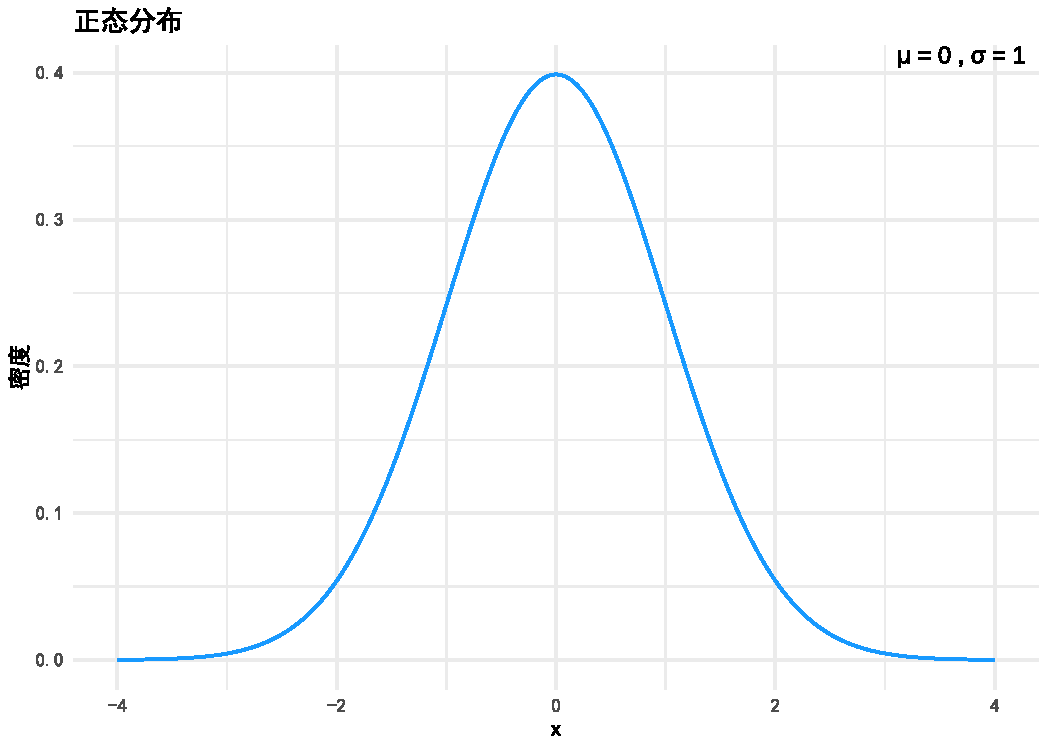
\includegraphics[width=\linewidth]{image/normal_distribution.pdf}}
		\subcaption{正态分布}
	\end{minipage}
	\hfill
	\begin{minipage}{0.48\textwidth}
		\centering
		\fbox{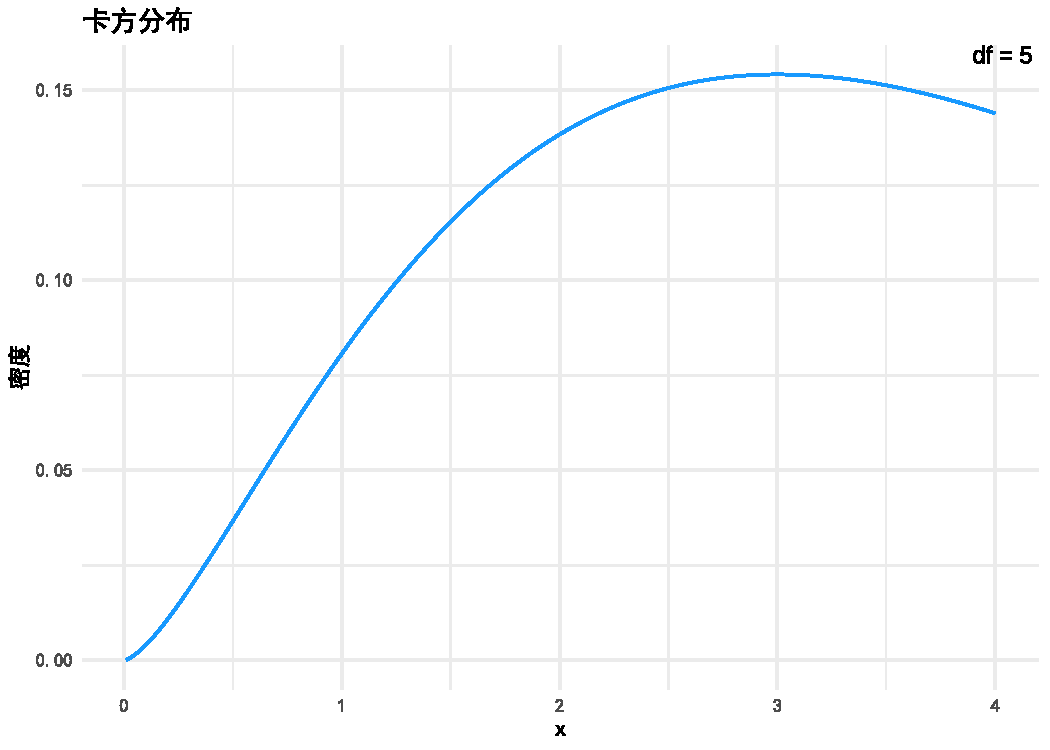
\includegraphics[width=\linewidth]{image/chi_squared_distribution.pdf}}
		\subcaption{卡方分布}
	\end{minipage}
	
	\vspace{1em}
	
	\begin{minipage}{0.48\textwidth}
		\centering
		\fbox{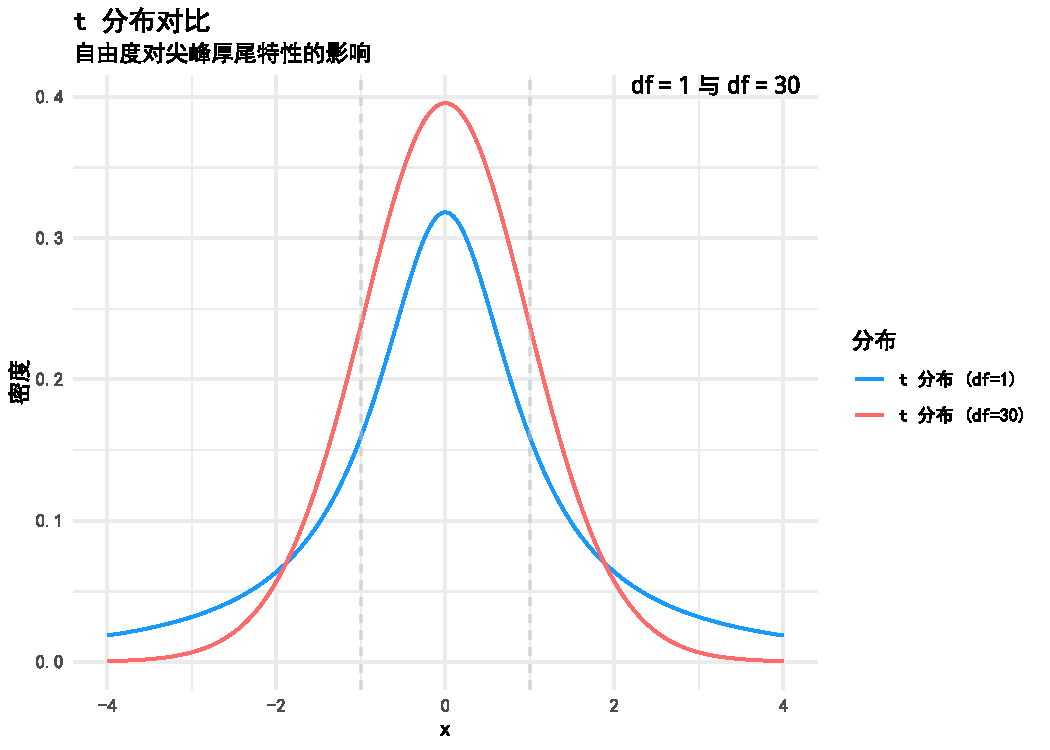
\includegraphics[width=\linewidth]{image/t_distribution_comparison.pdf}}
		\subcaption{$t$分布}
	\end{minipage}
	\hfill
	\begin{minipage}{0.48\textwidth}
		\centering
		\fbox{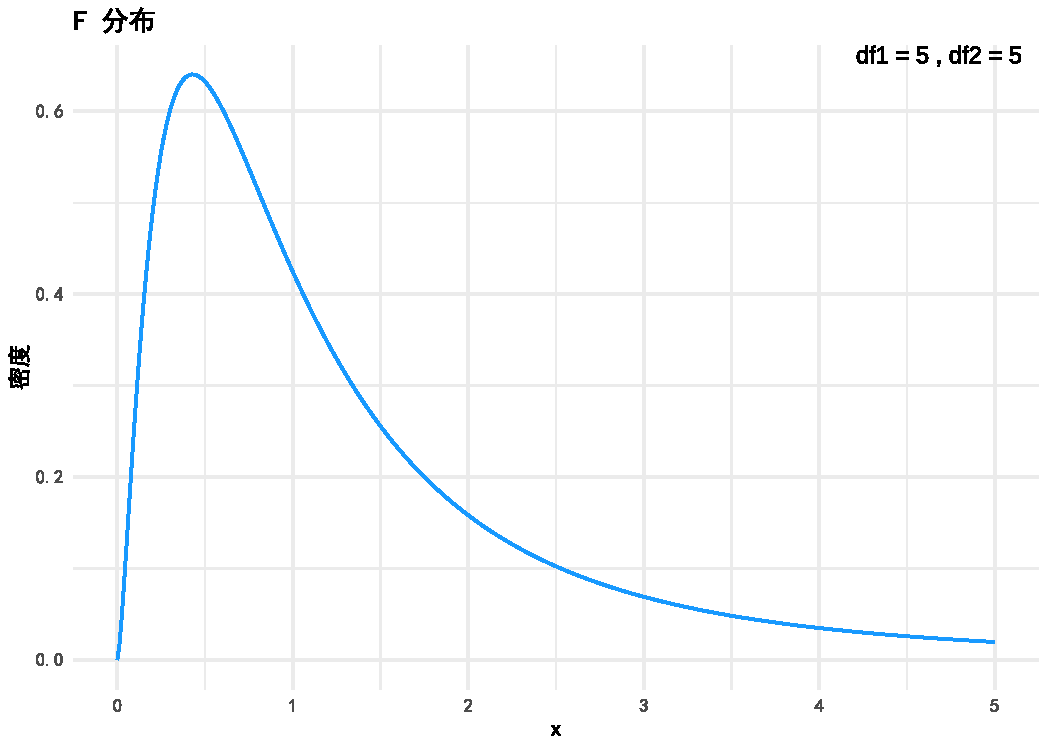
\includegraphics[width=\linewidth]{image/f_distribution.pdf}}
		\subcaption{$F$分布}
	\end{minipage}
	
	\caption{常见概率分布的比较}
	\label{fig:distributions}
\end{figure}

\subsection{统计推断的核心概念}

\paragraph*{总体与样本}
\begin{itemize}
	\item 总体(Population):研究对象的全体。
	\item 样本(Sample):从总体抽取的部分个体(容量$n$)。
	\item 理想样本:独立同分布(iid)随机样本。
\end{itemize}

\paragraph*{参数估计}
\begin{flushleft}
对于参数$\theta$,其估计量:
\end{flushleft}
\begin{equation}
	\hat{\theta} = \hat{\theta}(x_1,...,x_n) 
\end{equation}
\begin{itemize}
	\item 样本统计量(随机变量)。
	\item 估计值:给定样本时的具体取值。
\end{itemize}

\begin{flushleft}
常见估计量包括:
\end{flushleft}
\begin{align*}
	\text{样本均值} & : \bar{x} = \frac{1}{n}\sum x_i \\
	\text{样本中位数} & : \mathrm{median}(x_1,...,x_n) \\
	\text{极端值} & : \max/\min(x_1,...,x_n)
\end{align*}

\paragraph*{估计量的评价标准}
\begin{flushleft}
偏差的定义:
\end{flushleft}
\begin{equation}
	\mathrm{Bias}(\hat{\theta}) = E(\hat{\theta}) - \theta 
\end{equation}
当$E(\hat{\theta}) = \theta$时,称$\hat{\theta}$为无偏估计(unbias estimator),反之则为有偏估计(bias estimator)。

\paragraph*{均方误差(MSE)分解}
\begin{flushleft}
均方误差可以分解为方差与偏差平方之和:
\end{flushleft}
\begin{equation}
	\operatorname{MSE}(\hat{\theta})=\operatorname{Var}(\hat{\theta})+[\operatorname{Bias}(\hat{\theta})]^{2} 
\end{equation}

\begin{flushleft}
证明过程:
\end{flushleft}
\begin{equation}
	\begin{split}
		\operatorname{MSE}(\hat{\theta})&\equiv E\left[(\hat{\theta}-\theta)^{2}\right]\\
		&=E\left\{[\hat{\theta}-E(\hat{\theta})+E(\hat{\theta})-\theta]^{2}\right\} \\
		&=E\left[\hat{\theta}-E(\hat{\theta})\right]^{2}+2E\left\{[\hat{\theta}-E(\hat{\theta})][E(\hat{\theta})-\theta]\right\}+E[E(\hat{\theta})-\theta]^{2} \\
		&=\operatorname{Var}(\hat{\theta})+[\operatorname{Bias}(\hat{\theta})]^{2}
	\end{split}
\end{equation}

\begin{flushleft}
其中交叉项为0,因为:
\end{flushleft}
\begin{equation}
	E\{[\hat{\theta}-E(\hat{\theta})][E(\hat{\theta})-\theta]\}=[E(\hat{\theta})-\theta]\cdot 0=0 
\end{equation}

\paragraph*{偏差-方差权衡}
\begin{flushleft}
统计学的核心命题是均方误差可以分解为:
\end{flushleft}
\begin{equation}
	E\left[(\hat{\theta}-\theta)^{2}\right] = \underbrace{\mathrm{Bias}(\hat{\theta})^2}_{\text{近似误差}} + \underbrace{\mathrm{Var}(\hat{\theta})}_{\text{估计波动}} + \underbrace{\varepsilon}_{\text{随机误差}}
\end{equation}

\begin{flushleft}
极端案例对比:
\end{flushleft}
\begin{itemize}
	\item 无偏高方差估计量$\hat{\theta}$(如高阶多项式回归,易过拟合)
	\item 有偏低方差估计量$\tilde{\theta}$(如一次回归,可能欠拟合)
\end{itemize}

\begin{figure}[ht]
	\centering
	\fbox{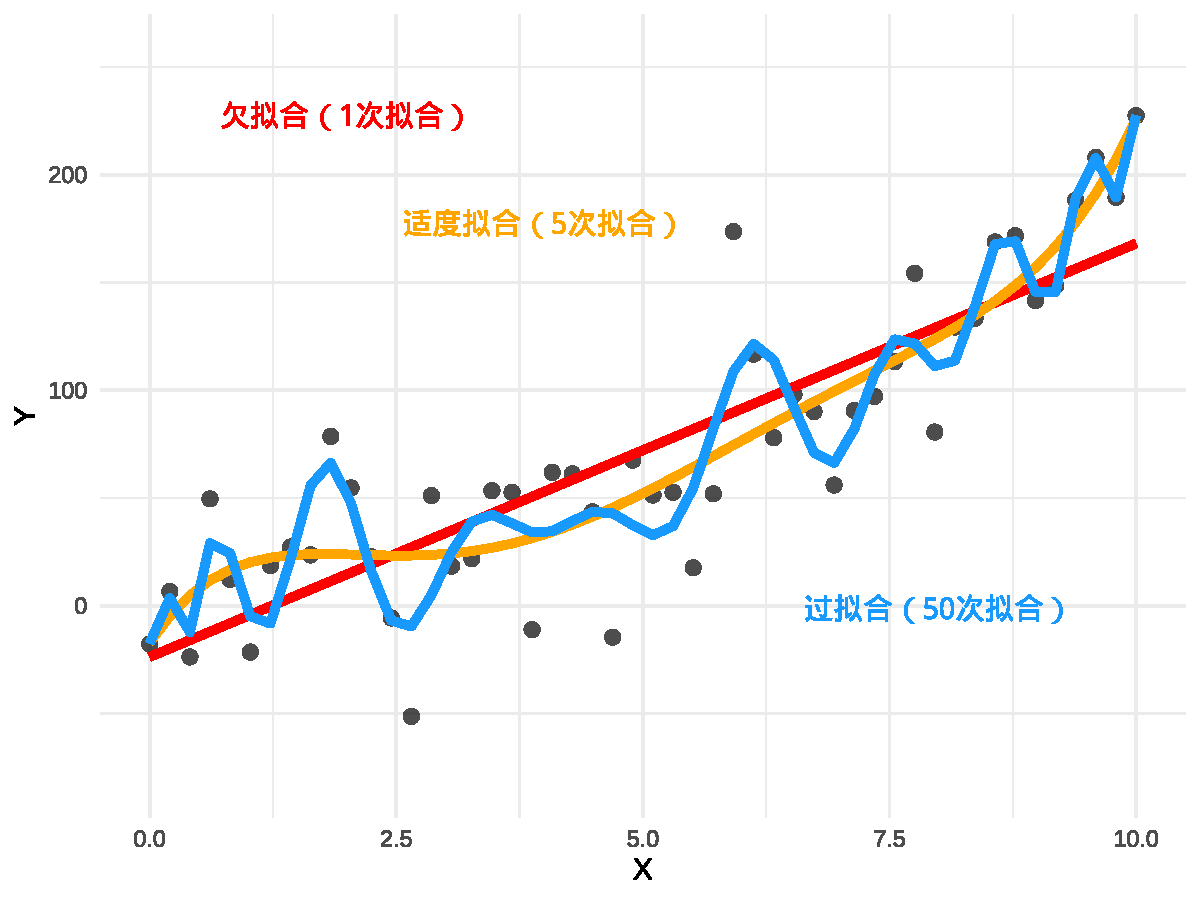
\includegraphics[width=0.5\linewidth]{image/fit_comparison}}
	\caption{拟合示例图}
\end{figure}

\section{社会科学中的统计推断}

\subsection{描述变量}

如何描述变量。这看似是一个简单的目标,但其内涵远比表面深刻。第二章讨论了如何建立研究问题,以及实证研究如何帮助我们理解世界,本章的前半部分回顾(预习)了基本的数学知识,此刻我们讨论变量描述。

实证研究问题本质上可归结为描述统计变量的密度分布——定量实证研究的核心就在于此。所有有趣的实证研究发现——无论是物理学、社会学、生物学、医学、经济学、政治学等领域——都有一条共同的主线。这条主线精巧地建立在概率基础之上,其形态表现为统计变量的密度分布,将整个宇宙中所有实证知识永恒地联系在一起。

为了理解数据,我们必须掌握如何观察并描述它们。这需要描述变量的类型及其分布形态。本节专注于单变量描述(后一节将讨论变量间的交互关系)。虽然单变量描述看似不如多变量分析有趣,但其重要性不容忽视。

在实证研究中,\textbf{变量}指对同一测量指标的一系列观测结果:如433名上海人的月收入、1999-2025年中国每年的企业并购数量、744名儿童的神经质心理评分、532朵花的颜色、《人民日报》上世纪某段时间内的头条新闻标题等。成功描述一个变量意味着能够清晰解释观测结果,而无需让他人查看所有原始数据。

\begin{flushleft}
描述变量的第一步是确定其类型。最常见的\textbf{变量类型}包括:
\end{flushleft}

\paragraph*{连续变量(Continuous Variables)}
连续变量可在一定范围内取任意值。例如上海人的月收入可以是12,000元,也可以是20,000元,或介于两者之间的任何值。这类变量没有``下一个最高''的概念,因为其变化是连续的。

\paragraph*{计数变量(Count Variables)}
计数变量记录事件发生的次数或物体的数量。例如中国每年的企业并购数量。计数变量不能为负值,也不能取分数值。当计数变量取值较多时,其性质接近连续变量,常被当作连续变量处理。

\paragraph*{有序变量(Ordinal Variables)}
有序变量的取值有``多''``少''之分,但缺乏精确的量化标准。例如神经质评分的``低''``中''``高''三个等级。虽然``高''高于``低'',但高多少并不明确。教育程度的``小学''``中学''``高中''``大学''也是有序变量——完成高中教育意味着比初中教育程度更高,但``高多少''无法精确量化。

\paragraph*{分类变量(Categorical Variables)}
分类变量记录观测对象所属的类别。例如花的颜色(白、橙、红)。这些类别没有高低之分,仅是不同类别。在社会科学研究中极为常见(如宗教信仰、种族、地理位置等)。\textbf{二元变量}是分类变量的特例,仅有两个取值(如``是/否'')。其优势在于便于处理实验效应(是否接受治疗),且多分类变量可转化为多个二元变量(如将政治面貌转化为``是否团员''``是否党员''等)。

\paragraph*{定性变量(Qualitative Variables)}
定性变量是非数值型、非分类的变量集合。如《人民日报》标题文本。这类变量通常包含大量难以概括的细节,常需转化为其他变量类型进行分析(如统计标题提及女性政治人物的次数,或使用AI模型进行特征评分)。

\begin{flushleft}
确定变量类型后,下一步是考察其\textbf{分布}——描述变量各取值出现概率的特征。
\end{flushleft}

\paragraph*{分布描述}
对于分类或有序变量,可通过给出各类别/取值的百分比来描述分布。完整分布可通过频率表或条形图展示。

\begin{table}[h]
	\centering
	\renewcommand{\arraystretch}{1.5}
	\caption{美国高校学位类型分布}
	\begin{tabularx}{1\linewidth}{>{\raggedright\arraybackslash}Xcc}
		\toprule
		授予的主要学位类型 & 数量(N) & 百分比(\%) \\
		\midrule
		两年制以下学位 & 3495 & 47 \\
		两年制学位 & 1647 & 22 \\
		四年制及以上学位 & 2282 & 31 \\
		总计 & 7424 & 100 \\
		\bottomrule
	\end{tabularx}
\end{table}

\begin{figure}[ht]
	\centering
	\fbox{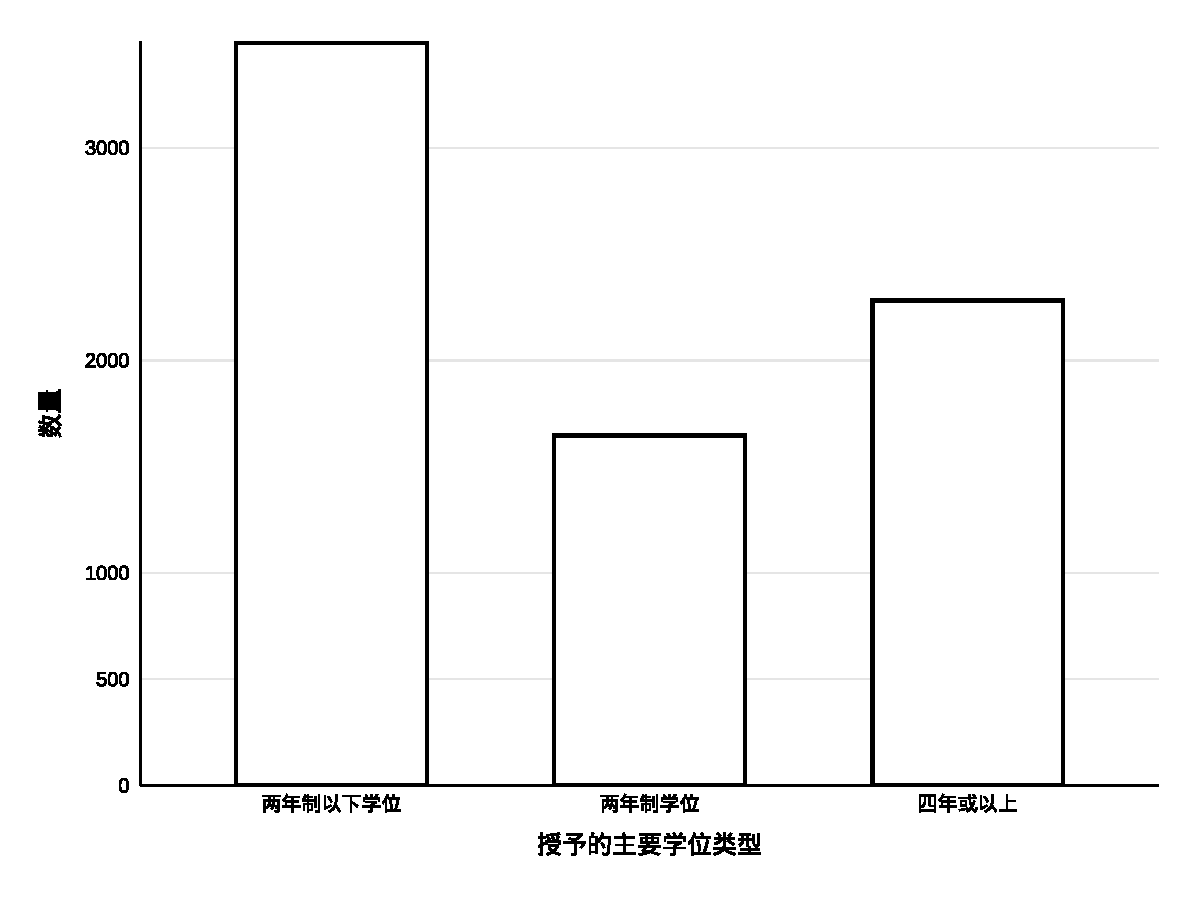
\includegraphics[width=0.5\textwidth]{image/earnings_distribution.pdf}}
	\caption{美国高校毕业生平均收入分布图}
	\label{fig:earnings}
\end{figure}


连续变量的分布描述更为复杂。由于观测值重复概率低,需采用\textbf{直方图}(将数据范围划分为区间并显示各区间的观测比例)或\textbf{密度图}(显示当直方图区间无限变窄时的极限形态)。密度曲线下面积代表概率,如图\ref{fig:earnings}所示,16\%的观测值位于40,000至50,000美元区间。

当完整分布信息量过大时(尤其对连续变量),需用少量数字概括分布特征。最经典的例子是\textbf{均值}——将所有观测值相加后除以观测数。均值代表数据的中心趋势,试图生成一个代表性数值。

\paragraph*{百分位数(Percentiles)}
\textbf{X百分位数}指X\%的观测值小于该值的点。例如身高数据的第5百分位数为5英尺4英寸。中位数(第50百分位数)是另一种中心趋势度量,代表典型观测值(对偏斜数据更稳健)。最小值和最大值(第0和100百分位数)显示变量的取值范围,其差值称为\textbf{极差}。

\paragraph*{变异度量}
变量间变异程度不同(如子女人数变异较大,而眼睛数量变异较小)。\textbf{方差}是基于均值的变异度量:
\begin{enumerate}
	\item 计算均值
	\item 各观测值减均值(得离均差)
	\item 离均差平方
	\item 求平方和
	\item 除以观测数减1(得样本方差)
\end{enumerate}

为消除平方单位影响,常取方差的平方根得\textbf{标准差}(恢复原始单位)。标准差有助于评估观测值的相对位置(如收入38,000美元者比均值高37.6\%个标准差)。

\paragraph*{四分位距(IQR)}是第75与25百分位数之差,覆盖样本中50\%最接近中位数的观测值,对极端值不敏感。

\paragraph*{偏度(Skew)}
偏度描述分布向一侧倾斜的程度。例如年收入分布有长右尾(少数极高收入者),称为\textbf{右偏}。左偏分布则有长左尾。对称分布则两侧尾部相近。

处理偏斜数据的常用方法是对数转换(使数据更接近正态分布)。自然对数转换的优势在于系数解释直观(对数增加0.01约对应原始变量1\%的增长)。

统计学严格区分\textbf{真相}(理论分布)与\textbf{数据}(观测分布)。我们真正关心的是理论分布(生成数据的分布),而非样本统计量。随着样本量增加,观测分布会趋近理论分布。

\paragraph*{常见理论分布}
\begin{itemize}
	\item \textbf{正态分布}:对称分布(如身高、智商)。即使严格意义上不适用(如身高不能为负),但当近似良好时仍被广泛采用。
	\item \textbf{对数正态分布}:取对数后呈正态分布的右偏分布(如收入、财富、公司规模等)。其优势在于可通过对数转换消除偏度。
\end{itemize}

\paragraph*{假设检验中的 \(H_0\) 和 \(H_1\)}

在统计推断中,假设检验是判断样本数据是否支持某一假设的核心方法。我们通常定义:
\[
\begin{cases}
H_0: \text{原假设(Null Hypothesis),一般表示无效假设或无差异}\\
H_1: \text{备择假设(Alternative Hypothesis),表示研究者关心的效应存在或差异存在}
\end{cases}
\]
检验的目标是基于样本数据决定是否拒绝 \(H_0\),从而间接支持 \(H_1\)。

\paragraph*{第一类错误与第二类错误}

由于样本具有随机性,假设检验不可避免地存在两种错误:

\begin{itemize}
	\item \textbf{第一类错误(``弃真''错误):} 当 \(H_0\) 为真时,错误地拒绝了 \(H_0\)。犯此错误的概率称为显著性水平 \(\alpha\)。
	\item \textbf{第二类错误(``取伪''错误):} 当 \(H_1\) 为真时,错误地未拒绝 \(H_0\)(即接受了错误的原假设)。犯此错误的概率用 \(\beta\) 表示。
\end{itemize}

显著性水平 \(\alpha\) 通常事先设定(如 0.05),用于控制第一类错误概率的上限。第二类错误概率 \(\beta\) 反映检验的``检验力''(Power),即正确拒绝错误的原假设 \(H_0\) 的能力,其值为 \(1-\beta\)(例如检验力为 0.95 表示有 95\% 的概率能够正确拒绝无效的原假设。)。

回顾第一章中波普尔的观点——科学中没有不能被质疑的陈述。科学普遍理论的基本命题必须是可证伪的,即应当能够通过实证加以检验和潜在的反驳。

在科学实践中,我们更倾向于积极检验理论,力图通过证据去反驳,而非轻易接受某个理论。因此,统计检验通常强调控制第一类错误(显著性水平 \(\alpha\)),以避免盲目拒绝真实理论。同时,在科学探索中,第一类错误的风险通常被视为较为可控的代价,而错误接受错误理论(第二类错误)可能更严重地阻碍科学进步。

因此,标准的统计推断做法是:只要样本数据提供的证据足够强(即 \(p\) 值小于预设的显著性水平 \(\alpha\)),就拒绝原假设 \(H_0\)。但需要明确的是,拒绝 \(H_0\) 并不意味着备择假设 \(H_1\) 必然为真,仅表明数据与 \(H_0\) 不符,支持 \(H_1\) 的可能性较大。统计推断本质上是概率性的,而非绝对确定。

\paragraph*{从数据推断理论分布}
我们可通过假设检验评估理论分布的可能性:
\begin{enumerate}
	\item 选择理论分布的某个特征(如均值$\mu$)
	\item 基于理论分布性质和样本量,确定该特征在随机样本中的抽样分布
	\item 计算观测数据的对应特征
	\item 评估观测结果在理论分布中的出现概率
	\item 若概率极低,则拒绝原理论分布假设
\end{enumerate}
	
\vspace{0.8em} % 手动调整间距

\begin{example}
	篮球运动员得分数据样本中有100个数据,得分均值为102,标准差为30($n=100$,$\bar{x}=102$,$s=30$),假设理论均值$\mu=90$成立吗?
	
\begin{flushleft}	
1. 抽样分布的推导
\end{flushleft}
根据中心极限定理(Central Limit Theorem, CLT),当样本大小 \(n\) 足够大时(一般 \(n \geq 30\)),样本均值的抽样分布近似正态分布:
\begin{itemize}
	\item 分布的均值等于总体均值(在 \(H_0\) 下,\(\mu = 90\))。
	\item 分布的标准差(称为标准误差,\(\sigma_{\bar{x}}\)) 由公式 \(\sigma_{\bar{x}} = \frac{s}{\sqrt{n}}\) 计算。
\end{itemize}

\begin{flushleft}
给定数据:n = 100, \quad s = 30
\end{flushleft}

\begin{flushleft}
计算标准误差:
\end{flushleft}
\begin{equation}
\sigma_{\bar{x}} = \frac{s}{\sqrt{n}} = \frac{30}{\sqrt{100}} = \frac{30}{10} = 3
\end{equation}
因此,在 \(H_0\) 下,样本均值的抽样分布是正态分布 \(N(90, 3)\)(即均值为 90,标准差为 3)。这可以写为:
\begin{equation}
\bar{X} \sim N(\mu, \sigma_{\bar{x}}^2) = N(90, 3^2) = N(90, 9)
\end{equation}
(注:\(N(\mu, \sigma^2)\) 表示正态分布,其中第二个参数是方差;标准差为 \(\sigma = 3\),方差为 \(\sigma^2 = 9\)。在推断中,通常直接使用标准差。)

\begin{flushleft}	
2. 检验统计量(z-分数)的计算
\end{flushleft}
观测样本均值 \(\bar{x} = 102\)。我们计算其与假设均值 \(\mu = 90\) 的差异,并以标准误差为单位标准化:
\begin{equation}
z = \frac{\bar{x} - \mu}{\sigma_{\bar{x}}} = \frac{102 - 90}{3} = \frac{12}{3} = 4
\end{equation}
z-分数为 4,表示观测均值 \(\bar{x} = 102\) 与假设均值 \(\mu = 90\) 相差 4 个标准误差(即 4 个标准差单位)。这反映了在 \(H_0\) 下,观测值的相对位置。

\begin{flushleft}	
3. p-值的解释
\end{flushleft}
p-值是在 \(H_0\) 成立时,观测到与样本均值一样极端或更极端结果的概率。这是一个双尾检验(因为 \(H_1: \mu \neq 90\)),因此:
\begin{equation}
\text{p-value} = P(|\bar{X}| \geq |\bar{x}| \mid H_0) \approx P(|Z| \geq 4) \quad \text{(其中 } Z \sim N(0,1)\text{)}
\end{equation}
在标准正态分布下:
\begin{itemize}
	\item \(P(Z \geq 4) \approx 0.00003167\)(右尾概率)。
	\item 双尾 p-值 \(\approx 2 \times 0.00003167 = 0.00006334\)。
\end{itemize}
因此,p-值远小于 0.0001(即 \(p < 0.0001\))。这表明,如果 \(H_0\) 为真(\(\mu = 90\)),观测到样本均值 \(\bar{x} = 102\)(或更极端)的概率极低(小于万分之一),属于统计学上的极端事件。

\begin{flushleft}
4. 结论
\end{flushleft}
给定显著性水平 \(\alpha = 0.05\)(常用阈值):
\begin{equation}
\text{p-value} < 0.0001 < 0.05 = \alpha
\end{equation}
因此,我们有非常强的证据拒绝原假设 \(H_0: \mu = 90\)。结论是:篮球运动员的平均得分不太可能是 90,更可能高于此值。

\end{example}

\subsection{描述关系}

对于大多数研究问题,我们不仅对单个变量的分布感兴趣,更关注数据中两个或多个变量之间的关系。两个变量之间存在关系意味着什么?这种关系显示了了解一个变量能为我们提供关于另一个变量的信息。

例如儿童的身高与年龄。通常,孩子年龄越大,身高越高。因此知道一个孩子13岁而另一个6岁,就能较好地猜测谁更高。我们可以称身高与年龄的关系为``正相关''——一个变量的较高值往往对应另一个变量的较高值(年龄越大身高越高)。也存在``负相关''关系(年龄越大哭闹越少),以及``零相关''关系(儿童年龄与居住可能性无关)。其他关系可能时正时负,或初期强正相关后期弱正相关。若变量是分类变量,则不存在``高低''之分,只有``差异''(大孩子更可能骑自行车上学)。

\paragraph*{条件分布}

上一章讨论的是变量的无条件分布(也称边缘分布)。条件分布则是指给定另一个变量特定值时,某个变量的分布。

以条件概率为例:随机一个人是女性的概率约50\%,但名叫\textbf{翠花}的人是女性的概率远高于50\%。我们称之为``在名为翠花的条件下是女性的概率''。条件分布同理,不过是从单一概率扩展到整个分布的变化。

图\ref{fig:vitaminE}展示了服用维生素E剂量的分布,按是否进行剧烈运动分组。可见运动者与非运动者的分布存在差异——运动者服用剂量更大。这种分布差异表明维生素E摄入与运动存在关联。

\begin{figure}[ht]
	\centering
	\fbox{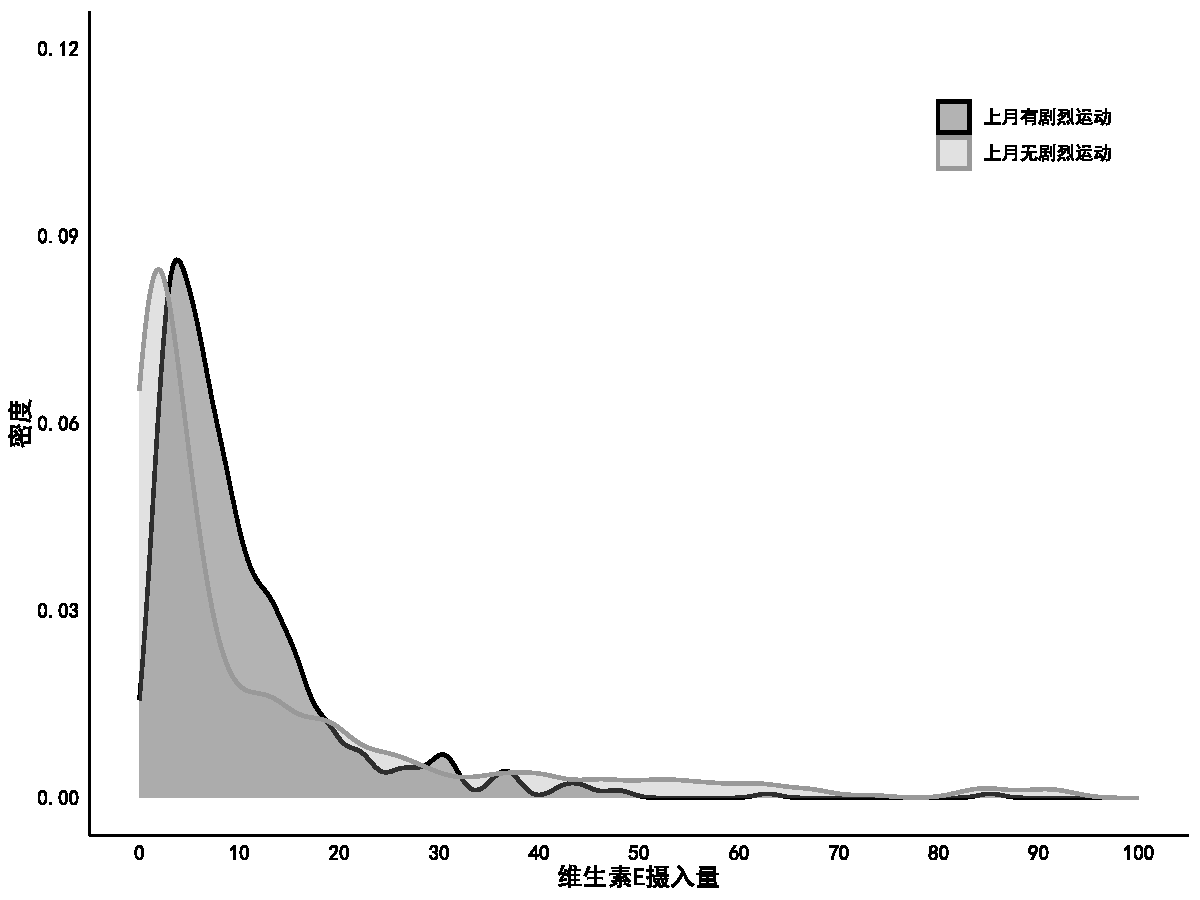
\includegraphics[width=0.5\textwidth]{image/vitaminE_density.pdf}}
	\caption{上月运动情况对维生素E摄入量的影响}
	\label{fig:vitaminE}
\end{figure}

该概念同样适用于分类变量。图\ref{fig:vitaminEbarchart}显示:不吸烟人群服用维生素E的比例明显高于吸烟人群,这与Oster关于健康意识驱动行为的假设一致。

\begin{figure}[ht]
	\centering
	\fbox{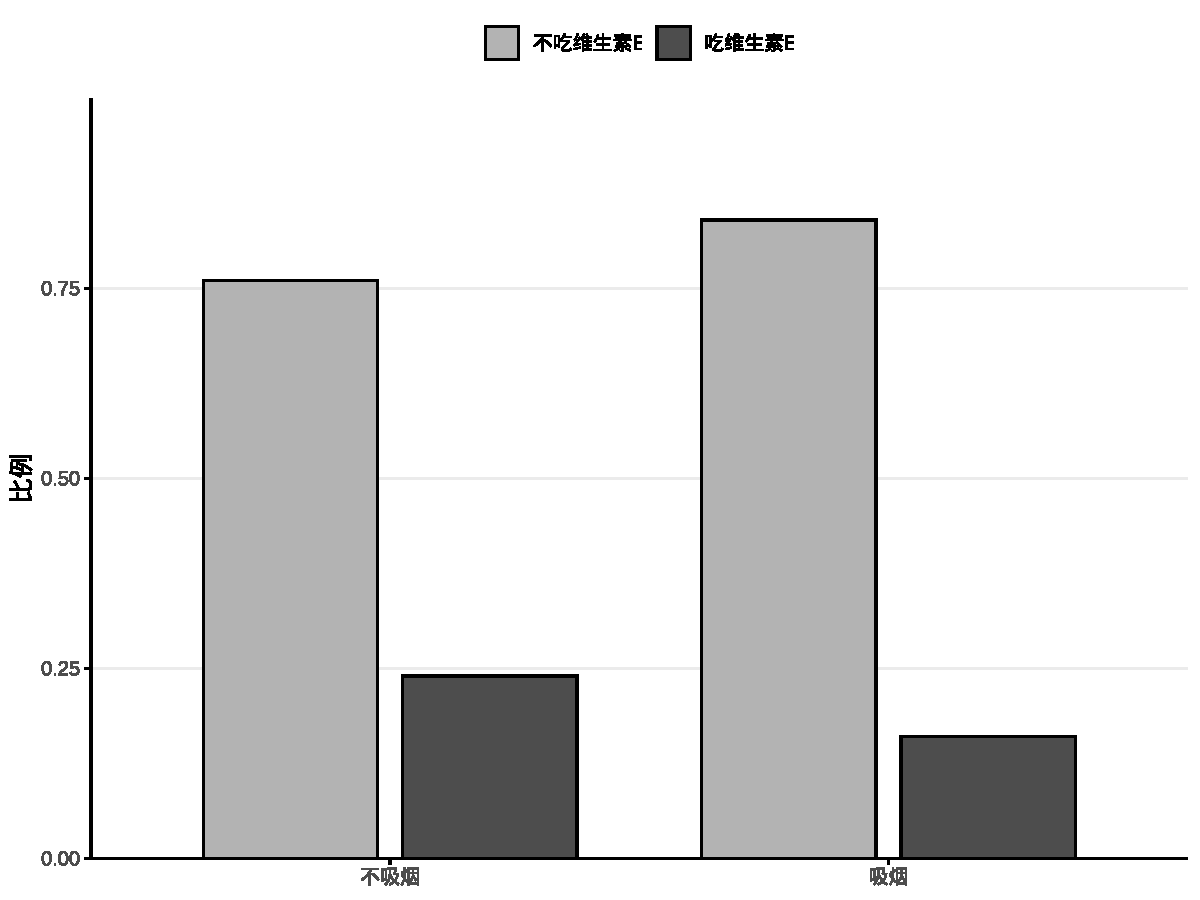
\includegraphics[width=0.5\textwidth]{image/vitaminE_barchart.pdf}}
	\caption{是否吸烟与是否服用维生素E的关系}
	\label{fig:vitaminEbarchart}
\end{figure}

\paragraph*{条件均值}

掌握条件分布概念后,我们可计算该分布的任何特征。本章重点讨论条件均值——给定变量$X$的特定值,变量$Y$的期望均值。

对于离散变量,计算简单:只需取该值所有观测的均值。图\ref{fig:VitaminE_by_BMI}显示维生素E服用比例随时间阶段(推荐前/中/后)的变化:推荐期间呈现正相关,推荐取消后转为负相关。

\begin{figure}[ht]
	\centering
	\fbox{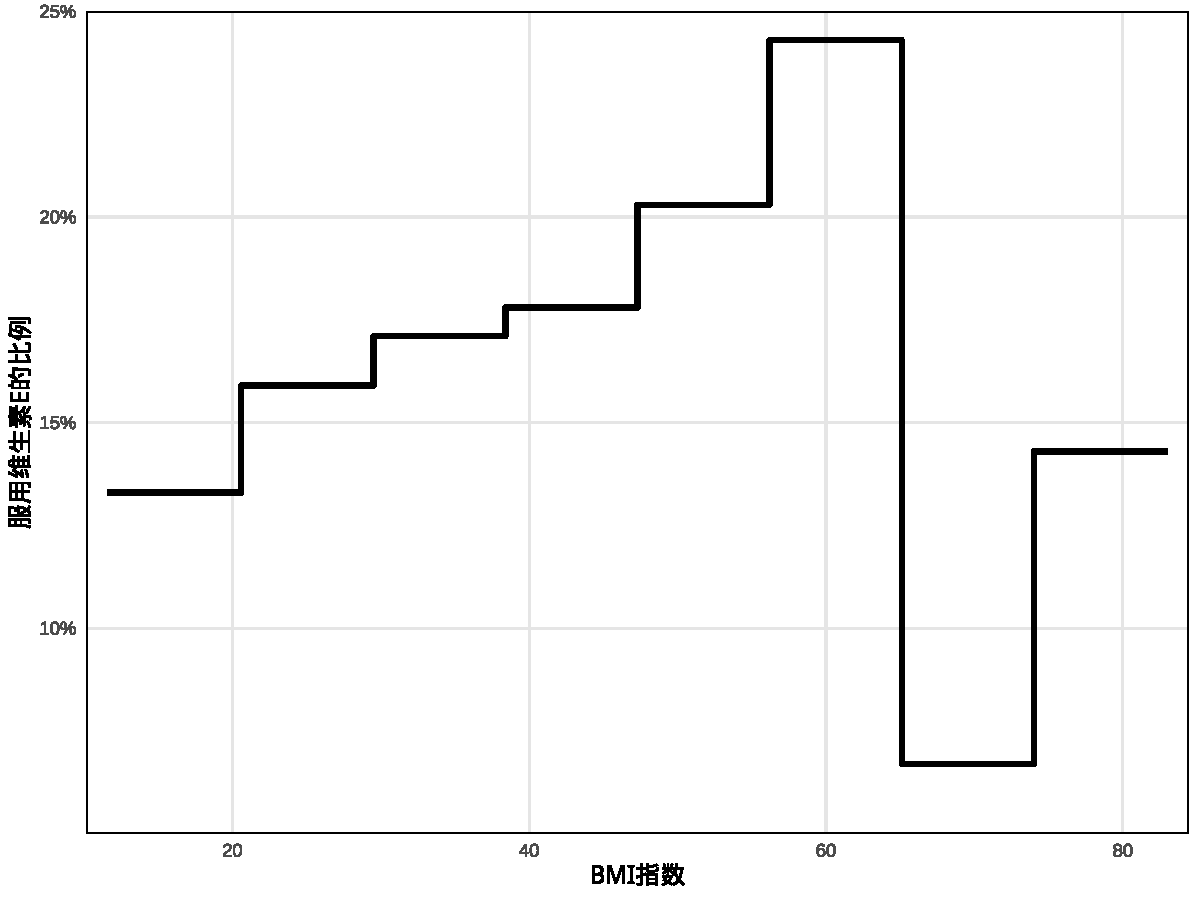
\includegraphics[width=0.5\textwidth]{image/VitaminE_by_BMI.pdf}}
	\caption{按体重指数值范围分列的服用维生素E的比例}
	\label{fig:VitaminE_by_BMI}
\end{figure}

连续变量则更复杂。解决方法有两种:
\begin{enumerate}
	\item 将连续变量划分为若干区间(分箱),计算各区间内均值
	\item 使用局部均值或LOESS曲线(局部加权散点平滑)进行平滑处理
\end{enumerate}

图\ref{fig:LOESS_Curve}的LOESS曲线清晰显示:BMI越高,维生素E服用率越高,初期关系强烈后期趋于平缓。这种方法通过移动窗口计算局部均值,避免分箱法的任意性缺陷。

\begin{figure}[ht]
	\centering
	\fbox{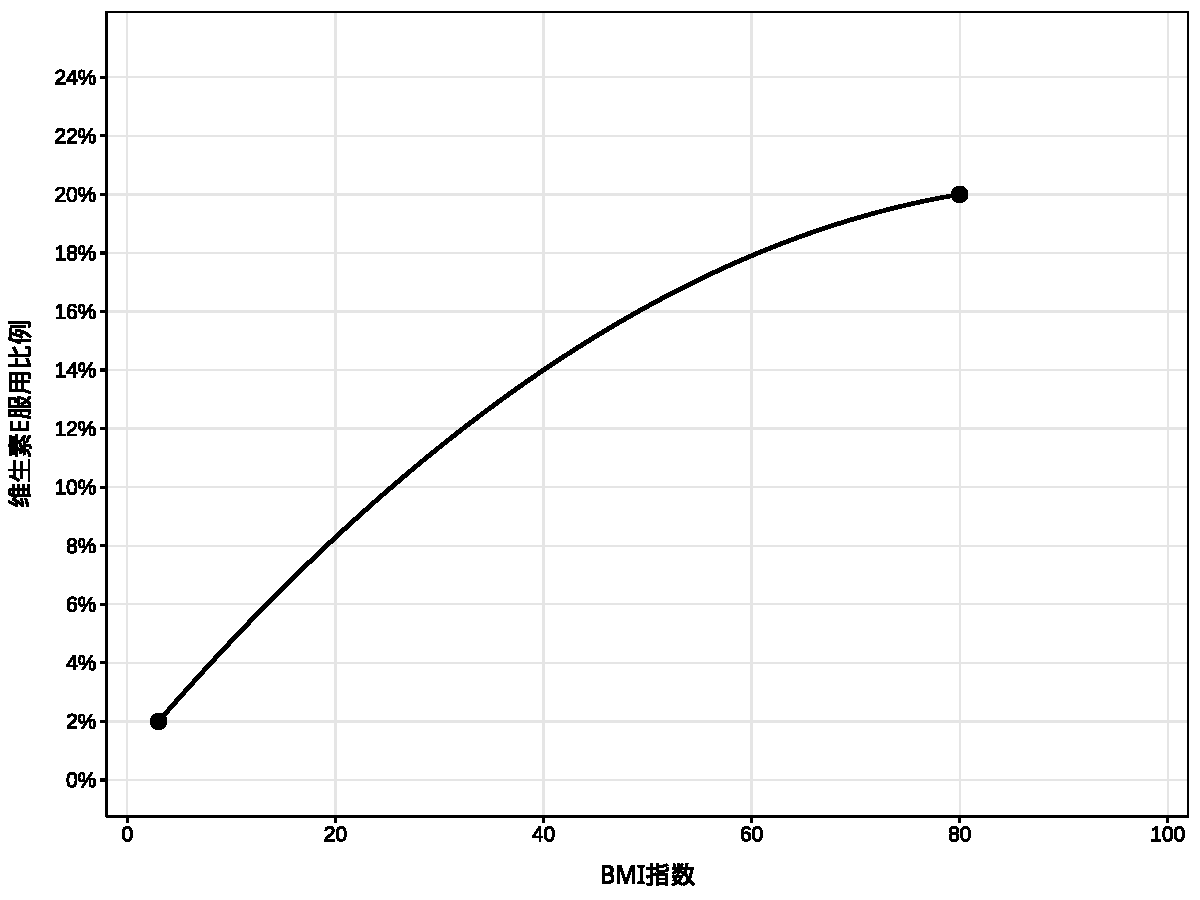
\includegraphics[width=0.5\textwidth]{image/LOESS_Curve.pdf}}
	\caption{按体重指数(BMI)划分的服用维生素 E 的比例(LOESS)曲线}
	\label{fig:LOESS_Curve}
\end{figure}

\paragraph*{回归分析}

另一种方法是假设变量间存在某种数学关系(通常是直线),即回归分析。图\ref{fig:VitaminE_BMI_linear}用直线拟合维生素E与BMI的关系,斜率0.002表示BMI每增加1单位,服用概率上升0.2个百分点。

\begin{figure}[ht]
	\centering
	\fbox{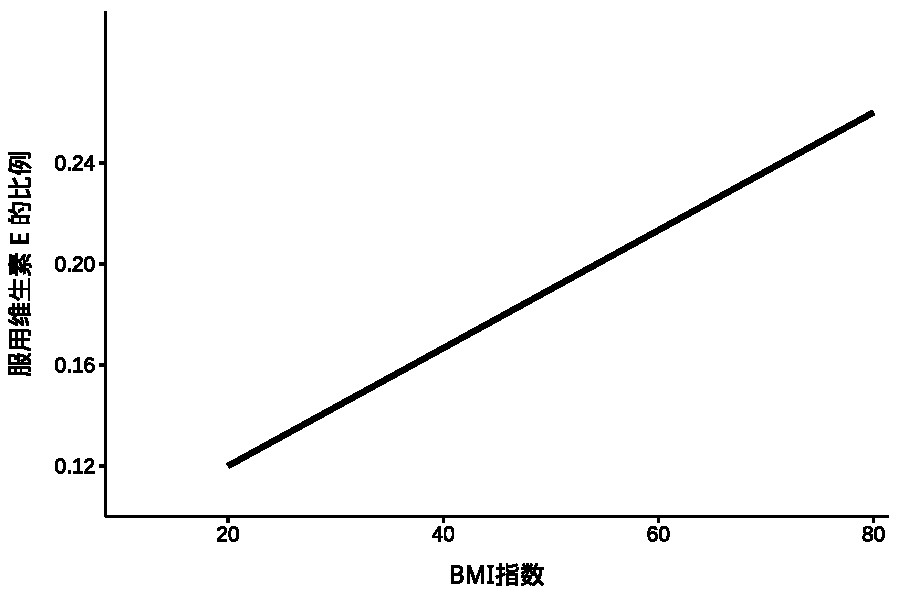
\includegraphics[width=0.5\textwidth]{image/VitaminE_BMI_linear.pdf}}
	\caption{用拟合直线表示按体重指数计算的服用维生素E的比例}
	\label{fig:VitaminE_BMI_linear}
\end{figure}

普通最小二乘法(OLS)是最常用的直线拟合方法,通过最小化残差平方和确定最佳直线。其斜率计算公式为协方差除以$X$的方差,直观反映了``$X$的变化中有多少与$Y$协同变化''。

当直线拟合不足时,可采用:
\begin{itemize}
	\item 多项式回归(如二次曲线)
	\item 非线性转换(如对数、概率单位转换)
\end{itemize}

\paragraph*{条件均值(``控制变量'')}

通过回归残差,我们可以剥离已解释部分,专注于未被解释的变异。将这个方法应用于双变量,就能实现``控制变量''——消除$Z$对$X$和$Y$的影响后,分析二者的纯净关系。

多元回归是最高效的实现方式,在仅考虑BMI时,我们估计:
\begin{equation}
	\text{VitaminE} = .110 + .002 \times \text{BMI}
\end{equation}

现在加入BMI、性别和年龄后,得到:
\begin{equation}
	\text{VitaminE} = -.006 + .001 \times \text{BMI} + .002 \times \text{Age} + .016 \times \text{Female}
\end{equation}

在控制年龄和性别后,BMI的效应从0.002降至0.001,说明原关系部分由这些变量解释。同时,年龄每增加1岁服用概率提高0.2个百分点,女性比男性高1.6个百分点。

这种方法在数学上对应Frisch-Waugh-Lovell定理:通过回归残差间的回归,等效于直接进行多元回归。这让我们能清晰分离不同变量的独立影响。

\newpage
\thispagestyle{empty}
\begin{thebibliography}{99}
	\bibitem{1}
	陈强,《计量经济学及Stata应用(第2版)》,高等教育出版社
	
	\bibitem{2}
	Nick Huntington-Klein,《The Effect》,CRC Press
	
\end{thebibliography}
